% Practice Test 11 — Texas Edition
% Questions: 30 (19 MC + 11 SA)
% Generated by scripts/generate_practice_tests.py

\begin{practiceQuestion}{1-3-q09}{mc}
\begin{questionText}
Find $k$ from the table.

\begin{center}
\begin{tabular}{|c|c|}
\hline $x$ & $y$ \\ \hline $6$ & $9$ \\ $10$ & $15$ \\ $14$ & $21$ \\ \hline
\end{tabular}
\end{center}
\end{questionText}
\choiceA{$1.5$}
\choiceB{$3$}
\choiceC{$\frac{2}{3}$}
\choiceD{$6$}
\correctAnswer{A}
\explanation{$k = \frac{9}{6} = 1.5$. Check: $\frac{15}{10} = 1.5$ and $\frac{21}{14} = 1.5$.}
\end{practiceQuestion}

\begin{practiceQuestion}{1-6-q11}{mc}
\begin{questionText}
A train travels $315$ miles in $4.5$ hours. At this rate, how far does it travel in $7$ hours?
\end{questionText}
\choiceA{$420$ miles}
\choiceB{$455$ miles}
\choiceC{$490$ miles}
\choiceD{$525$ miles}
\correctAnswer{C}
\explanation{Rate: $315 \div 4.5 = 70$ mph. In $7$ hours: $70 \times 7 = 490$ miles.}
\end{practiceQuestion}

\begin{practiceQuestion}{2-1-q13}{mc}
\begin{questionText}
Which proportion can be used to find $30\%$ of $90$?
\end{questionText}
\choiceA{$\dfrac{n}{90} = \dfrac{30}{100}$}
\choiceB{$\dfrac{30}{n} = \dfrac{90}{100}$}
\choiceC{$\dfrac{90}{n} = \dfrac{30}{100}$}
\choiceD{$\dfrac{n}{100} = \dfrac{30}{90}$}
\correctAnswer{A}
\explanation{The part $n$ is over the whole $90$, and the percent $30$ is over $100$: $\frac{n}{90} = \frac{30}{100}$.}
\end{practiceQuestion}

\begin{practiceQuestion}{2-3-q08}{mc}
\begin{questionText}
A computer originally costs $\$600$. After a $15\%$ price drop, what is the new price?
\end{questionText}
\choiceA{$\$90$}
\choiceB{$\$510$}
\choiceC{$\$515$}
\choiceD{$\$585$}
\correctAnswer{B}
\explanation{Multiply by $1 - 0.15 = 0.85$: $600 \times 0.85 = \$510$.}
\end{practiceQuestion}

\begin{practiceQuestion}{2-6-q03}{mc}
\begin{questionText}
In the formula $I = Prt$, what does $P$ represent?
\end{questionText}
\choiceA{The percent rate}
\choiceB{The principal (starting amount)}
\choiceC{The interest earned}
\choiceD{The time in years}
\correctAnswer{B}
\explanation{$P$ stands for principal, which is the starting amount of money deposited or borrowed.}
\end{practiceQuestion}

\begin{practiceQuestion}{2-8-q09}{mc}
\begin{questionText}
You buy a $\$120$ jacket. Using a debit card costs $\$120$. Using a credit card at $15\%$ annual interest (paid after $1$ year) costs how much total?
\end{questionText}
\choiceA{$\$120$}
\choiceB{$\$135$}
\choiceC{$\$138$}
\choiceD{$\$150$}
\correctAnswer{C}
\explanation{Interest $= 120 \times 0.15 = \$18$. Total $= 120 + 18 = \$138$.}
\end{practiceQuestion}

\begin{practiceQuestion}{2-9-q09}{mc}
\begin{questionText}
Your food budget is $\$300$ per month. You spend $\$330$ one month. By what percent did you go over budget?
\end{questionText}
\choiceA{$10\%$}
\choiceB{$3\%$}
\choiceC{$30\%$}
\choiceD{$11\%$}
\correctAnswer{A}
\explanation{Over by $\$30$. Percent: $\frac{30}{300} = 0.10 = 10\%$.}
\end{practiceQuestion}

\begin{practiceQuestion}{2-10-q08}{mc}
\begin{questionText}
Deposit $\$600$ at $10\%$ for $2$ years. How much MORE does compound interest earn compared to simple interest?
\end{questionText}
\choiceA{$\$6$}
\choiceB{$\$12$}
\choiceC{$\$120$}
\choiceD{$\$60$}
\correctAnswer{A}
\explanation{Simple: $I = 600 \times 0.10 \times 2 = \$120$, total $= \$720$. Compound: Year 1: $660$; Year 2: $660 \times 1.10 = \$726$. Difference: $726 - 720 = \$6$.}
\end{practiceQuestion}

\begin{practiceQuestion}{4-1-q27}{gmc}
\begin{questionText}
The diagram below represents an algebraic expression using algebra tiles.

\begin{center}
\begin{tikzpicture}[scale=0.6]
  % x-tiles (rectangles)
  \fill[funBlue!40] (0,0) rectangle (2,1);
  \draw[thick] (0,0) rectangle (2,1);
  \node at (1,0.5) {$x$};
  \fill[funBlue!40] (2.5,0) rectangle (4.5,1);
  \draw[thick] (2.5,0) rectangle (4.5,1);
  \node at (3.5,0.5) {$x$};
  \fill[funBlue!40] (5,0) rectangle (7,1);
  \draw[thick] (5,0) rectangle (7,1);
  \node at (6,0.5) {$x$};
  % unit tiles (squares)
  \fill[funGreen!40] (8,0) rectangle (9,1);
  \draw[thick] (8,0) rectangle (9,1);
  \node at (8.5,0.5) {$1$};
  \fill[funGreen!40] (9.5,0) rectangle (10.5,1);
  \draw[thick] (9.5,0) rectangle (10.5,1);
  \node at (10,0.5) {$1$};
\end{tikzpicture}
\end{center}

Which expression do the tiles represent?
\end{questionText}
\choiceA{$3x + 2$}
\choiceB{$2x + 3$}
\choiceC{$5x$}
\choiceD{$3x \times 2$}
\correctAnswer{A}
\explanation{There are $3$ $x$-tiles and $2$ unit tiles. The expression is $3x + 2$.}
\end{practiceQuestion}

\begin{practiceQuestion}{4-2-q30}{gsa}
\begin{questionText}
The table shows the number of each type of tile in a bag. Write a simplified expression for the total number of tiles.

\begin{center}
\begin{tabular}{|l|c|}
\hline
\textbf{Tile Color} & \textbf{Number of Tiles} \\
\hline
Red & $3n + 4$ \\
\hline
Blue & $2n - 1$ \\
\hline
Green & $n + 5$ \\
\hline
Yellow & $4n - 2$ \\
\hline
\end{tabular}
\end{center}
\end{questionText}
\correctAnswer{$10n + 6$}
\explanation{Add all expressions: $(3n + 4) + (2n - 1) + (n + 5) + (4n - 2)$. Combine variable terms: $3n + 2n + n + 4n = 10n$. Combine constants: $4 - 1 + 5 - 2 = 6$. Total: $10n + 6$.}
\end{practiceQuestion}

\begin{practiceQuestion}{5-3-q22}{sa}
\begin{questionText}
Solve $2(x + 7) = -6$.
\end{questionText}
\correctAnswer{$x = -10$}
\explanation{Divide by $2$: $x + 7 = -3$. Subtract $7$: $x = -10$. Check: $2(-10 + 7) = 2(-3) = -6$ \checkmark.}
\end{practiceQuestion}

\begin{practiceQuestion}{5-4-q16}{mc}
\begin{questionText}
A student estimates that the solution to $0.48x + 3.1 = 12.7$ is about $x = 20$. Is this estimate reasonable?
\end{questionText}
\choiceA{Yes, the exact answer is $20$}
\choiceB{Yes, the exact answer is close to $20$}
\choiceC{No, the exact answer is about $10$}
\choiceD{No, the exact answer is about $33$}
\correctAnswer{A}
\explanation{Subtract $3.1$: $0.48x = 9.6$. Divide by $0.48$: $x = 20$. The estimate is exactly correct.}
\end{practiceQuestion}

\begin{practiceQuestion}{5-5-q04}{mc}
\begin{questionText}
Solve $5x - 10 \geq 25$.
\end{questionText}
\choiceA{$x \geq 3$}
\choiceB{$x \geq 7$}
\choiceC{$x \leq 7$}
\choiceD{$x \geq 35$}
\correctAnswer{B}
\explanation{Add $10$: $5x \geq 35$. Divide by $5$: $x \geq 7$.}
\end{practiceQuestion}

\begin{practiceQuestion}{5-6-q14}{mc}
\begin{questionText}
Solve $-3x + 12 \geq 0$ and describe the graph.
\end{questionText}
\choiceA{Closed circle at $4$, shade right}
\choiceB{Open circle at $4$, shade left}
\choiceC{Closed circle at $4$, shade left}
\choiceD{Closed circle at $-4$, shade right}
\correctAnswer{C}
\explanation{Subtract $12$: $-3x \geq -12$. Divide by $-3$ and flip: $x \leq 4$. Closed circle at $4$, shade left.}
\end{practiceQuestion}

\begin{practiceQuestion}{6-2-q20}{sa}
\begin{questionText}
A map uses $1$ cm $= 100$ km. You redraw at $1$ cm $= 25$ km. A distance is $3$ cm on the original. How long is it on the new map?
\end{questionText}
\correctAnswer{$12$ cm}
\explanation{Scale ratio: $\frac{100}{25} = 4$. New length: $3 \times 4 = 12$ cm.}
\end{practiceQuestion}

\begin{practiceQuestion}{6-3-q26}{gmc}
\begin{questionText}
Look at the three segments below. Can they form a triangle?

\begin{center}
\begin{tikzpicture}
  \draw[thick,funBlue] (0,0) -- (2,0);
  \node[below] at (1,0) {$2$ cm};
  \draw[thick,funBlue] (0,-1) -- (3,-1);
  \node[below] at (1.5,-1) {$3$ cm};
  \draw[thick,funBlue] (0,-2) -- (6,-2);
  \node[below] at (3,-2) {$6$ cm};
\end{tikzpicture}
\end{center}
\end{questionText}
\choiceA{Yes, exactly one triangle}
\choiceB{Yes, more than one triangle}
\choiceC{No, because $2 + 3 < 6$}
\choiceD{No, because the sides are all different lengths}
\correctAnswer{C}
\explanation{$2 + 3 = 5 < 6$. The two shorter sides cannot reach across the longest, so no triangle can be formed.}
\end{practiceQuestion}

\begin{practiceQuestion}{6-4-q29}{gsa}
\begin{questionText}
Look at the triangle below. Two sides and the included angle are given. What is the condition type, and is the triangle unique?

\begin{center}
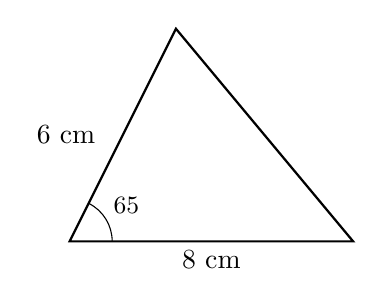
\begin{tikzpicture}[scale=0.9]
  \draw[thick] (0,0) -- (4,0) -- (1.5,3) -- cycle;
  \node[below] at (2,0) {$8$ cm};
  \node[left] at (0.5,1.5) {$6$ cm};
  \draw (0.6,0) arc[start angle=0,end angle=63,radius=0.6];
  \node at (0.8,0.5) {\small $65°$};
\end{tikzpicture}
\end{center}
\end{questionText}
\correctAnswer{SAS; yes, the triangle is unique}
\explanation{Two sides ($8$ cm and $6$ cm) and the included angle ($65°$) give the SAS condition. SAS always produces exactly one unique triangle.}
\end{practiceQuestion}

\begin{practiceQuestion}{6-5-q30}{gsa}
\begin{questionText}
The diagram shows a cube with edge length $6$ cm. A diagonal cut is made from vertex $A$ through the center to the opposite vertex $B$, passing through four faces. What type of shape could this cross-section be?

\begin{center}
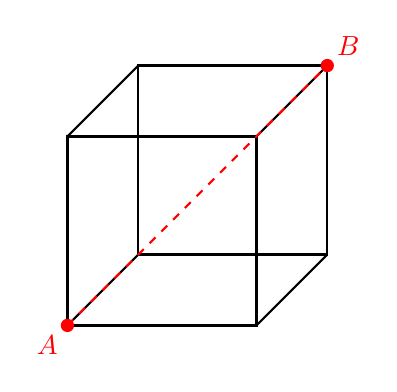
\begin{tikzpicture}[scale=0.6]
  % Front face
  \draw[thick] (0,0) -- (4,0) -- (4,4) -- (0,4) -- cycle;
  % Back face
  \draw[thick] (1.5,1.5) -- (5.5,1.5) -- (5.5,5.5) -- (1.5,5.5) -- cycle;
  % Connecting edges
  \draw[thick] (0,0) -- (1.5,1.5);
  \draw[thick] (4,0) -- (5.5,1.5);
  \draw[thick] (4,4) -- (5.5,5.5);
  \draw[thick] (0,4) -- (1.5,5.5);
  % Diagonal vertices
  \fill[red] (0,0) circle (4pt) node[below left] {$A$};
  \fill[red] (5.5,5.5) circle (4pt) node[above right] {$B$};
  % Diagonal line
  \draw[thick,red,dashed] (0,0) -- (5.5,5.5);
\end{tikzpicture}
\end{center}
\end{questionText}
\correctAnswer{A rectangle}
\explanation{A diagonal cut from one vertex of a cube to the opposite vertex, passing through four faces, creates a rectangular cross-section. The rectangle's dimensions are a face diagonal ($6\sqrt{2}$ cm) by the edge length ($6$ cm).}
\end{practiceQuestion}

\begin{practiceQuestion}{6-8-q07}{mc}
\begin{questionText}
Rectangle $ABCD \sim$ Rectangle $EFGH$. $AB = 6$, $BC = 10$, $EF = 9$. Find $FG$.
\end{questionText}
\choiceA{$13$}
\choiceB{$15$}
\choiceC{$18$}
\choiceD{$90$}
\correctAnswer{B}
\explanation{Scale factor: $\frac{9}{6} = 1.5$. $FG = 10 \times 1.5 = 15$.}
\end{practiceQuestion}

\begin{practiceQuestion}{7-4-q03}{mc}
\begin{questionText}
A shape is made of two rectangles. Rectangle A is $6$ m by $3$ m and Rectangle B is $4$ m by $3$ m. What is the total area?
\end{questionText}
\choiceA{$18$ m$^2$}
\choiceB{$24$ m$^2$}
\choiceC{$30$ m$^2$}
\choiceD{$72$ m$^2$}
\correctAnswer{C}
\explanation{Rectangle A: $6 \times 3 = 18$ m$^2$. Rectangle B: $4 \times 3 = 12$ m$^2$. Total: $18 + 12 = 30$ m$^2$.}
\end{practiceQuestion}

\begin{practiceQuestion}{7-5-q25}{sa}
\begin{questionText}
A rectangular prism has dimensions $4$ m, $4$ m, and $10$ m. How much greater is its surface area than a cube with side $4$ m?
\end{questionText}
\correctAnswer{$96$ m$^2$}
\explanation{Prism: $SA = 2(4 \times 4) + 2(4 \times 10) + 2(4 \times 10) = 32 + 80 + 80 = 192$ m$^2$. Cube: $6 \times 16 = 96$ m$^2$. Difference: $192 - 96 = 96$ m$^2$.}
\end{practiceQuestion}

\begin{practiceQuestion}{7-6-q10}{mc}
\begin{questionText}
A rectangular prism has a base area of $24$ cm$^2$ and a height of $7$ cm. What is its volume?
\end{questionText}
\choiceA{$31$ cm$^3$}
\choiceB{$168$ cm$^3$}
\choiceC{$336$ cm$^3$}
\choiceD{$17$ cm$^3$}
\correctAnswer{B}
\explanation{$V = Bh = 24 \times 7 = 168$ cm$^3$.}
\end{practiceQuestion}

\begin{practiceQuestion}{8-1-q25}{sa}
\begin{questionText}
A factory produces $10{,}000$ batteries per day. A sample of $200$ batteries is tested, and $8$ are defective. What percent of the sample is defective?
\end{questionText}
\correctAnswer{$4\%$}
\explanation{$\frac{8}{200} = 0.04 = 4\%$.}
\end{practiceQuestion}

\begin{practiceQuestion}{8-2-q07}{mc}
\begin{questionText}
In a random sample of $40$ students, $12$ said they prefer reading over video games. If the school has $500$ students, predict how many prefer reading.
\end{questionText}
\choiceA{$12$}
\choiceB{$120$}
\choiceC{$150$}
\choiceD{$200$}
\correctAnswer{C}
\explanation{$\frac{12}{40} = 30\%$. Then $30\%$ of $500 = 150$.}
\end{practiceQuestion}

\begin{practiceQuestion}{8-4-q23}{sa}
\begin{questionText}
Data: $100, 200, 300, 400, 500$. Find the median and the IQR.
\end{questionText}
\correctAnswer{Median $= 300$; IQR $= 200$}
\explanation{Median (3rd value) $= 300$. $Q_1 = 200$, $Q_3 = 400$. IQR $= 400 - 200 = 200$.}
\end{practiceQuestion}

\begin{practiceQuestion}{8-5-q19}{sa}
\begin{questionText}
Create a stem-and-leaf plot for: $32, 35, 41, 43, 47, 50, 52, 58$. What are the stems?
\end{questionText}
\correctAnswer{Stems: $3, 4, 5$}
\explanation{Stem $3$: leaves $2, 5$. Stem $4$: leaves $1, 3, 7$. Stem $5$: leaves $0, 2, 8$.}
\end{practiceQuestion}

\begin{practiceQuestion}{8-6-q25}{sa}
\begin{questionText}
A class of $50$ students: $20$ prefer summer, $15$ prefer winter, $10$ prefer fall, $5$ prefer spring. What percent prefer fall?
\end{questionText}
\correctAnswer{$20\%$}
\explanation{$\frac{10}{50} = 0.20 = 20\%$.}
\end{practiceQuestion}

\begin{practiceQuestion}{9-4-q28}{gmc}
\begin{questionText}
Look at the two bags below. Which bag represents a uniform probability model for drawing a marble?

\begin{center}
\begin{tikzpicture}[scale=0.65]
  % Bag 1
  \draw[thick,rounded corners=8pt] (-3,-1.5) rectangle (0,1.5);
  \node[above,font=\bfseries] at (-1.5,1.5) {Bag 1};
  \fill[funRed] (-2.3,0.5) circle (0.3);
  \fill[funRed] (-1.5,0.5) circle (0.3);
  \fill[funBlue] (-0.7,0.5) circle (0.3);
  \fill[funBlue] (-2.3,-0.5) circle (0.3);
  \fill[funGreen] (-1.5,-0.5) circle (0.3);
  \fill[funGreen] (-0.7,-0.5) circle (0.3);
  % Bag 2
  \draw[thick,rounded corners=8pt] (1,-1.5) rectangle (4,1.5);
  \node[above,font=\bfseries] at (2.5,1.5) {Bag 2};
  \fill[funRed] (1.7,0.5) circle (0.3);
  \fill[funRed] (2.5,0.5) circle (0.3);
  \fill[funRed] (3.3,0.5) circle (0.3);
  \fill[funRed] (1.7,-0.5) circle (0.3);
  \fill[funBlue] (2.5,-0.5) circle (0.3);
  \fill[funGreen] (3.3,-0.5) circle (0.3);
\end{tikzpicture}
\end{center}
\end{questionText}
\choiceA{Bag 1 only}
\choiceB{Bag 2 only}
\choiceC{Both bags}
\choiceD{Neither bag}
\correctAnswer{A}
\explanation{Bag 1 has $2$ of each color ($2$ red, $2$ blue, $2$ green), so each color is equally likely — uniform. Bag 2 has $4$ red, $1$ blue, $1$ green — non-uniform.}
\end{practiceQuestion}

\begin{practiceQuestion}{9-6-q17}{mc}
\begin{questionText}
Two spinners are spun. Spinner 1 has sections $\{1, 2, 3\}$ and Spinner 2 has sections $\{A, B\}$. What is the probability of getting $2$ and $A$?
\end{questionText}
\choiceA{$\frac{1}{3}$}
\choiceB{$\frac{1}{5}$}
\choiceC{$\frac{1}{6}$}
\choiceD{$\frac{2}{6}$}
\correctAnswer{C}
\explanation{$P(2) = \frac{1}{3}$, $P(A) = \frac{1}{2}$. $P = \frac{1}{3} \times \frac{1}{2} = \frac{1}{6}$.}
\end{practiceQuestion}

\begin{practiceQuestion}{9-7-q19}{sa}
\begin{questionText}
A simulation uses a coin flip ($50\%$ chance) to model whether it rains on a given day. In $30$ trials, rain occurs $16$ times. What is the experimental probability of rain?
\end{questionText}
\correctAnswer{$\frac{16}{30}$}
\explanation{$P = \frac{16}{30} \approx 0.533$.}
\end{practiceQuestion}
